\section{Stage 3: Explainable and Auditable Rankings}
The last stage of MERIT takes place once we have finished computing metrics for all of the candidates in the job configuration.
In this stage, we translate the complex internal mathematical states into transparent human-readable audit trails, as well as
simple visualisations to aid readability and understanding. MERIT's aim of being a glass-box recruitment system depends upon this stage,
as we need to ensure that recruiters are not just given a final score, but also the quantitative reasoning behind that score to either
trust, or even challenge candidate scores. We aid this by also providing probabilistic confidence scoring, applying Cooperative Game
Theory for data source contributions both to the candidate's final score, as well as to their individual metrics.

\subsection{Metric Confidence}
As mentioned in the previous chapter, Bayesian Evidence Fusion not only provides an expected value, but also a variance, in other words,
the certainty of that candidate's score. Two candidates may have a similar expected score for a metric, but could have vastly different
levels of confidence due to the sources of information for that metric. For example, one candidate may have verified signals across multiple
sources, while another candidate may only have a single, unverified claim from a low-trust source. It is important that a recruiter is able
to know of this, and in a simple manner.

We defined how variance is computed in section 4.3.4. We build upon this by now computing the confidence interval for that candidate's score.
Firstly, we calculate the standard deviation as $\sigma = \sqrt{\text{Var}(\theta)}$ to quantify this uncertainty. In our implementation of
MERIT, we avoid displaying confidence intervals to avoid cognitive overload for the recruiter. Instead, we express our confidence in a candidate's
score by outputting a label: ``High Confidence'', ``Medium Confidence'', or ``Low Confidence''.

We define ``High Confidence'' as a standard deviation $\sigma < 0.275$, ``Medium Confidence'' as $0.275 \le \sigma < 0.35$, and
``Low Confidence'' as $\sigma \ge 0.35$.

By outputting intuitive labels, rather than raw intervals, recruiters can quickly scan whether a candidate's score is
backed by a variety of strong evidence.


\subsection{Data Source Attribution}
While Bayesian Evidence Fusion and confidence scoring address the problem of understanding a candidate's proficiencies, we must address
the biggest disadvantage of this approach. Bayesian Evidence Fusion, at its core, is an aggregation mechanism that fuses multiple signals
together. We lose key information about the impact of each data source on that metric's final score. We cannot tell if a candidate got a high
score due to one very strong signal, or due to many weak signals. This is a problem that shatters the ``Glass-Box'' goal of MERIT, so it's vital
that we address this.

In a true ``Glass-Box'' system, recruiters must be able to understand the reasoning behind the scores, whether this was driven by demonstrated
evidence or claimed evidence. To solve this, we turn towards cooperative game theory, namely Shapley values. When data sources contain
overlapping or redundant signals, naive percentage breakdowns fail to accurately share credit amongst data sources. Shapley values
overcome this through a mathematically rigorous method of fairly distributing the total ``payoff'' (the candidate's score) amongst the
cooperating ``players'' (the data sources) \cite{shapley1953, lundberg2017unified}.

MERIT's implementation currently supports three sources of evidence. This is the candidate CV, GitHub and LinkedIn, therefore, we 
have $n = 3$ data sources. We create a set of all possible coalitions of data sources, computing the value of each coalition, 
denoted as $v(S)$ for a given subset of data sources $S$. For a set of sources $N$, we have $2^n$ possible coalitions, where $n$
refers to the number of data sources. In our case, this means $2^3 = 8$ possible coalitions. To compute the Shapley value $\phi_i$
for a given source $i$, we sum the marginal contributions of that source across all of the coalitions that it is a part of, as formally defined by Equation~\ref{eq:shapley_value}.

By calculating this Shapley value ($\phi_i$) for individual metrics and also for the final score, MERIT is able to attribute every score
to a data source, not just the final score. Now MERIT can inform the recruiter whether that score was driven by demonstrated evidence, or claimed evidence. Consequently,
this attribution remains consistent across all levels of abstraction. Data source contributions are fully traceable from the lowest-level 
signals up to the final aggregate match score.

\begin{figure}[htbp]
    \centering
    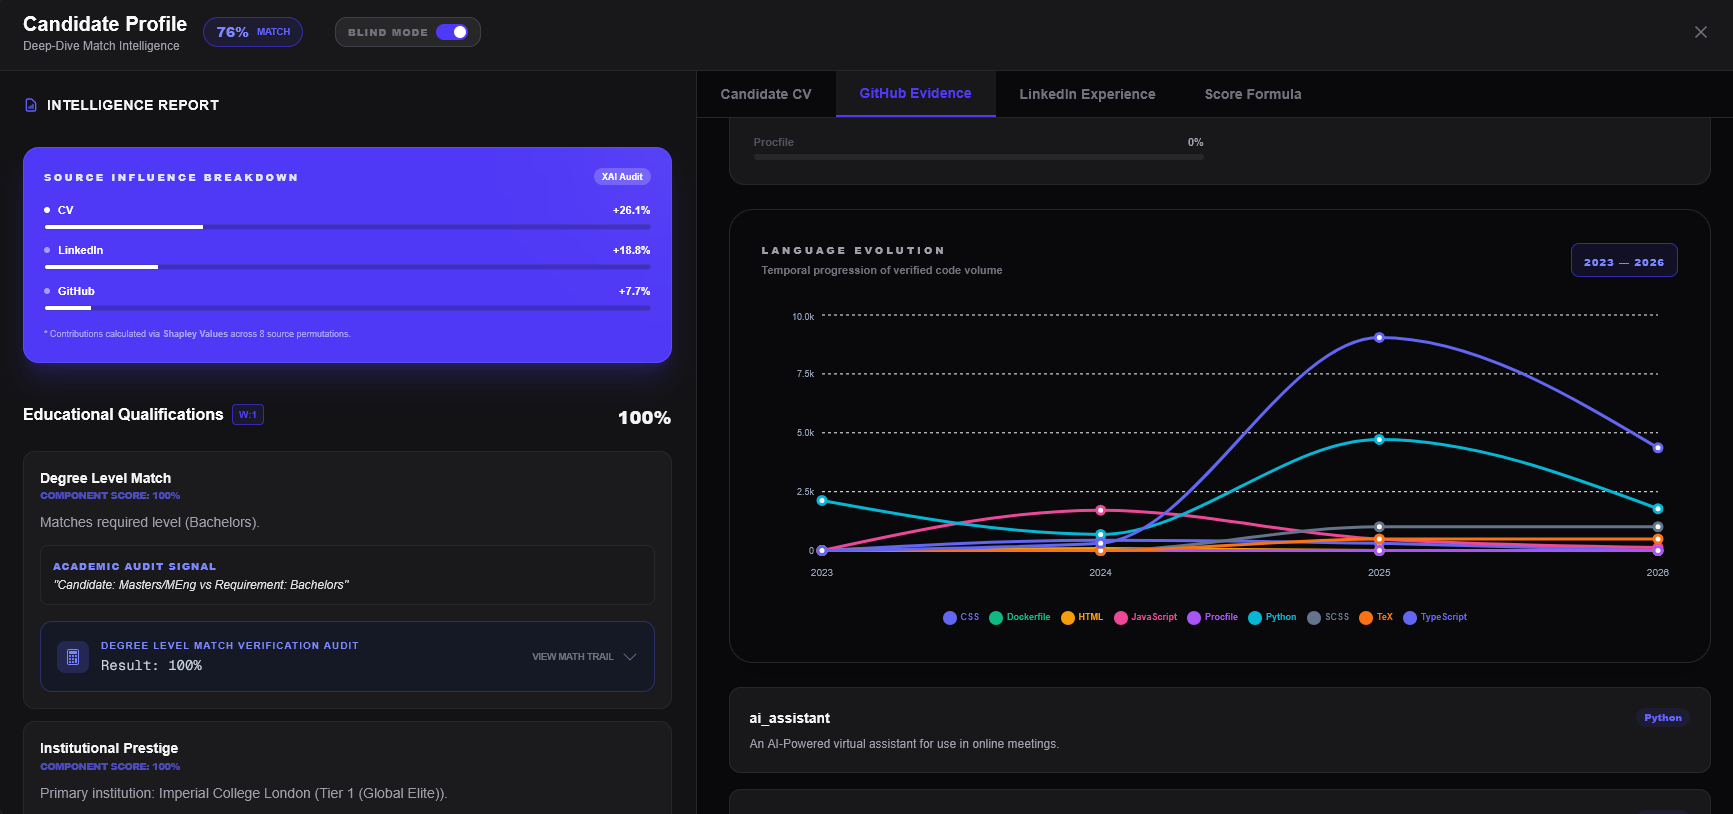
\includegraphics[width=0.95\textwidth]{implementation/screenshots/shapley_source_breakdown.png}
    \caption[Source Influence Breakdown panel]{Source influence breakdown with Shapley values per data source. In this figure,
    we show Shapley breakdown for the final match score. Shapley values for a specific metric can be viewed by clicking the ``View Math Trail''
    button}
    \label{fig:shapley_attribution}
\end{figure}


\subsection{Algorithmic Contestability}
MERIT also follows the principle of algorithmic contestability to further combat the black-box nature of these platforms.
We provide the specific evidence signals that were used to derive the score, this means that the full mathematical 
trail is provided to the recruiter to ensure that they can understand the reasoning behind the score. This in-depth
transparency is a focus of MERIT to allow recruiters to identify and override any algorithmic edge cases, or perhaps
see why a candidate got a penalisation, rather than letting this penalty go unnoticed. We ensure that the final decision
remains auditable, and aim to mitigate algorithmic bias.

The previous stage of MERIT (the execution phase) constructs both a \texttt{calculation\_summary} as well as a \texttt{results\_payload}.
For each metric, we provide the full breakdown, explicitly documenting every calculation that was performed to derive the score,
along with brief explanations for each step. Please refer to Appendix \ref{appendix:math_trail} 
for a complete step-by-step visualisation of the audit trail of an extensible metric.

This ``Glass-Box'' approach attempts to bridge the gap between complex probabilistic mathematics and practical recruitment
workflows, transforming a binary hiring decision into a defensible and interrogable process.


\subsection{Relative Cohort Normalisation}
Another common flaw with algorithmic scoring is the absence of relative context. A candidate with a year of experience may seem
weak on paper, but would be considered exceptional if the majority of the applicant pool had little to no experience. However, due
to this, the candidate would likely be undervalued if the system does not correctly highlight the difference in experience between
the candidate and the rest of the pool. To address this, MERIT also implements a dynamic cohort normalisation mechanism for the majority of
baseline metrics.

In order to achieve dynamic cohort normalisation, MERIT undergoes a two-pass approach. During the first pass of this stage, the backend
calculates the raw, absolute metrics for every candidate in the batch (such as Years of Experience, or Total GitHub repositories). Then
we aggregate these results to identify cohort maximums. In the second pass, we rerun the scoring engine, normalising candidate metrics against
the batch maximums. This approach, while not runtime efficient for extremely large datasets, ensures that MERIT's rankings remain adaptive
to the competitive landscape, rather than an arbitrary baseline.

\subsection{Glass-Box Dashboard}
\label{subsec:glass-box-dashboard}
Understandably, presenting the raw JSON \textit{results\_payload} is unreasonable due to it being inherently unscalable and poor UX.
We will briefly go over the main features of our Next.js frontend to create an intuitive, visual ``Glass-Box'' dashboard.

The first feature is probabilistic confidence labels, derived from the standard deviation $\sigma$ of the Beta distribution mentioned
in the previous chapter. We map $\sigma$ to a traffic-light badge system (Green for High, Amber for Medium, Red for Low),
allowing recruiters to instantly scan the reliability of a candidate's metric at a glance.
Non-critical penalties (e.g.\ keyword stuffing) show an amber icon on the ranking table, critical penalties (e.g.\ identity squatting) show a red warning. The significance of these labels is highlighted
more so when it comes to extensible metrics, where there is more uncertainty due to the ambiguity of how such metrics may be defined,
and calculated.

Another key innovation towards the UX of MERIT is the ``Insights'' panel. When viewing the ranking tables of a candidate, recruiters can open
a ``report'' for them, which will provide them with an overlay of, not only the candidate's score, but also how it was calculated. The metric's
calculation is also provided as a human-readable string, which can be used to understand the logic behind the score.
The panel links to the full audit trail (per-source signals, Bayesian fusion, and Shapley breakdown) and surfaces actionable 
guidance where scores are limited.
Figure~\ref{fig:glass-box-dashboards} shows the ranking table with confidence 
badges and the per-metric Insights overlay (full-size screenshots in Appendix~\ref{appendix:glass-box-ui}).

\begin{figure}[htbp]
    \centering
    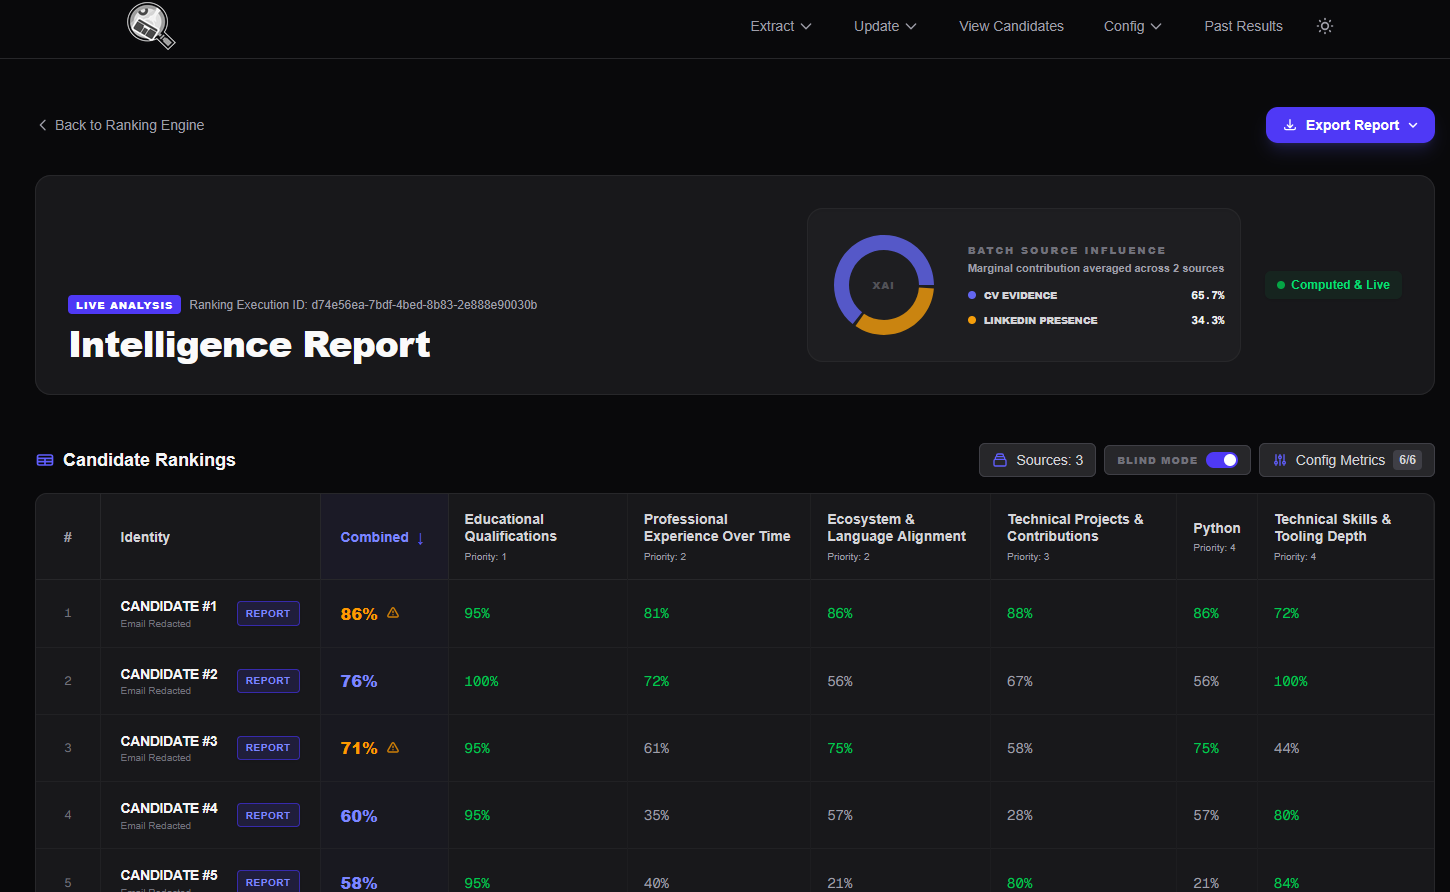
\includegraphics[height=0.17\textheight,keepaspectratio]{implementation/screenshots/candidate_rankings_dashboard.png}%
    \hfill
    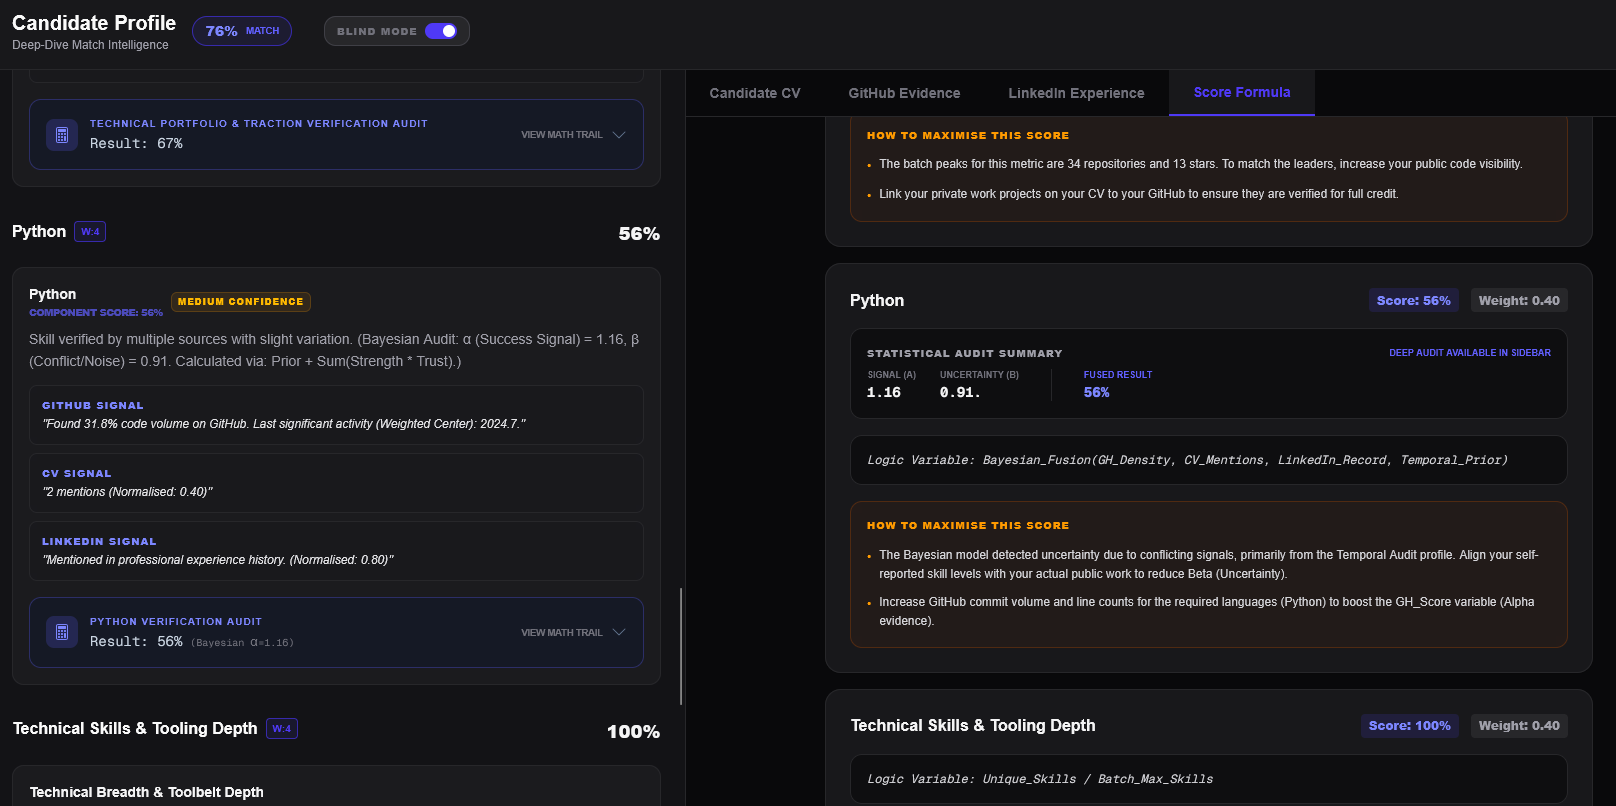
\includegraphics[height=0.17\textheight,keepaspectratio]{implementation/screenshots/metric_insights_panel.png}
    \caption[Glass-Box dashboard]{Glass-Box dashboard: Intelligence Report ranking table with confidence badges 
    (left) and Metric Insights panel for Python with audit trail (right). 
    Appendix~\ref{appendix:glass-box-ui} provides full-size versions.}
    \label{fig:glass-box-dashboards}
\end{figure}

To further aid transparency, any penalisations (such as Squatting) are also flagged to the user to highlight the negative impact of such actions on the candidate's score.
To ensure full auditability, we also provide views of each candidate's extracted data sources, so that recruiters can cross-check the audit trail.
It is also possible to view skillsets that may not have been considered by the scoring engine, for example, a configuration may have had Python
as a metric, but the candidate may have extensive work with Jupyter Notebook on their GitHub profile. If the semantic bridge mechanism fails to 
catch this, the recruiter would be able to still observe this data and potentially change their decision after accounting for this information.
